\documentclass{beamer}

\graphicspath{ {../Figures/} }

\usecolortheme[named=default]{}
\usetheme{Dresden}
\title[]{Distributed PowerShell Load Generator}
\subtitle[]{(D-PLG)}
\author[CSCE 689: Final Project]{Lt Paul Jordan and Lt Chip Van Patten}
\institute[D-PLG]{CSCE 689: Final Project}
\date{\today} 

\begin{document}

\frame{\titlepage} 

\frame{
  \frametitle{Overview}
  \tableofcontents
} 

\section{Introduction} 
\frame{
  \frametitle{Abstract} 
  \begin{itemize}
  \item Failure in cloud infrastructure is common occurrence
  \item Problem is often masked by the use of excessively redundant systems
  \item Machine learning techniques have been studied to predict
  failure~\cite{salfnerSurvey}
  \item Unfortunately, this work has gone unused~\cite{irrera2015}
  \end{itemize}
}

\frame{
  \frametitle{Solution?} 
  \begin{itemize}
  \item Framework introduced to solve problem called Adaptive Failure
  Prediction (AFP) Framework
  \item Load a service $\Rightarrow$ Inject faults $\Rightarrow$ Record failure
  \item How do we load a Microsoft Windows active directory domain?
  \end{itemize}
}

\frame{
  \frametitle{D-PLG} 
  \begin{itemize}
  \item PowerShell script
  \item Remote execution
  \item Full-stack two-way dynamic authentication traffic
  \item Full-stack simulated web browsing
  \item Dynamic file sharing
  \item \dots and so much more!
  \end{itemize}
}
  
\section{Related Work} 
\frame{
  \frametitle{Existing Tools} 
  \begin{itemize}
  \item Many software tools exist for generating network traffic\\
    Three major categories~\cite{botta2012,zach2013}:
    \begin{itemize}
    \item Application-Level
    \item Flow-Level
    \item Packet-Level
    \end{itemize}
  \item Unfortunately, no existing tools generate full-stack dynamic traffic
  which we need to generate real authentication traffic to sufficiently load a
  domain controller
  \end{itemize}
}

\section{D-PLG} 
\subsection{Overview}
\frame{
  \frametitle{D-PLG}
  \begin{figure}[H] \centering 
      \caption[Concept Diagram]{How each type of traffic that is generated is
      routed.  Log events are offloaded to logging service for further
      analysis.}
      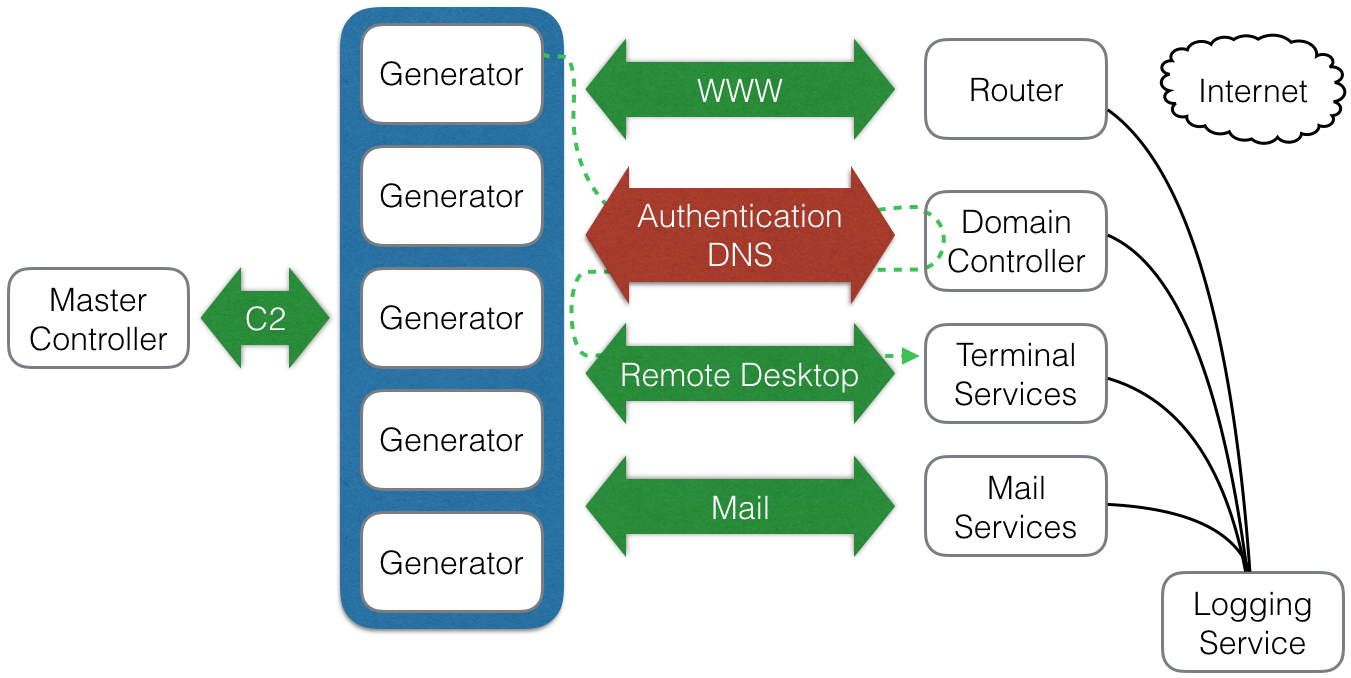
\includegraphics[width=2.8in]{ConceptDiagram}
      \label{fig:conceptDiagram} 
  \end{figure}
}

\subsection{Modules}
\frame{
  \frametitle{Web Browsing}
  \begin{itemize}
  \item PowerShell cmdlet `Invoke-WebRequest'
  \item Returns full DOM object
  \item Allows us to simulate browsing
  \end{itemize}
} 
\frame{
  \frametitle{Remote Desktop Protocol}
  \begin{itemize}
  \item Custom PowerShell cmdlet `Connect-Mstsc'~\cite{brasser15} 
  \item Hidden window so we don't interrupt users
  \item Makes connection, sleeps for a few seconds and then disconnects
  \item Plan to implement machine interaction
  \end{itemize}
} 
\frame{
  \frametitle{Server Message Block (SMB) File Sharing}
  \begin{itemize}
  \item PowerShell cmdlet `New-PSDrive'
  \item Connects and authenticates to remote file share
  \item Uploads 100 bytes of random ASCII data
  \item Deletes created file and disconnects
  \end{itemize}
} 

\frame{
  \frametitle{Future Modules}
  \begin{itemize}
  \item PowerShell cmdlet `Send-MailMessage'
  \item PowerShell cmdlet `Out-Printer'
  \end{itemize}
} 

\section{Methodology}
\frame{
  \centering
  \Huge Methodology
}

\subsection{Experiment Design}
\frame{
  \frametitle{Experiment}
  \begin{itemize}
  \item Two hypotheses:
    \begin{enumerate}
    \item We can sufficiently load the domain controller using our script
    \item We can use D-PLG without the end-user noticing
    \end{enumerate}
  \item Two tests: each five, five minute rounds of execution
  \item First test maximized traffic generated
  \item Second test balanced traffic generation with client utilization
  \item Capture all network traffic and performance/utilization metrics
  \end{itemize}
} 

\subsection{Virtual Environment}
\frame{
  \frametitle{Virtual Environment}
  \begin{figure}[H] \centering
    \caption{Hypervisor 1.}
    \begin{tabular}{ | c | l | l | c | l |}
      \hline
      Qty. & Role   & Operating System  & CPU / Mem. \\ \hline\hline
      1    & DC     & Win. Server 2008  & 2 / 2 GB   \\ \hline
      5    & Client & Win. 7            & 1 / 512 MB \\ 
      \hline
    \end{tabular}
    \label{fig:hyp1}
  \end{figure}

  \begin{figure}[H] \centering
    \caption{Hypervisor 2.}
    \begin{tabular}{ | c | l | l | c | l |}
      \hline
      Qty. & Role & Operating System  & CPU / Mem. \\ \hline\hline
      1    & RDP  & Win. Server 2008  & 1 / 4 GB   \\ \hline
      1    & Log  & Ubuntu 14.04 LTS  & 1 / 1 GB   \\ 
      \hline
    \end{tabular}
    \label{fig:hyp2}
\end{figure}

} 

\section{Experimental Results}
\frame{
  \centering
  \Huge Results
}
\subsection{First Test}
\frame{
  \frametitle{Results}
  \begin{itemize}
  \item First test was successful
  \item Able to sufficiently load domain controller based on Microsoft's
  community recommendations (15,000 clients authentication requests over five
  minutes).
  \end{itemize}
}
\frame{
  \frametitle{Results}
  \begin{figure}[H] \centering
    \caption[Domain Controller Packets per Second]{How many packets per second
    were sent or received by the domain controller across all five rounds of the
    first test.  In each test, we captured approximately 1.8 million packets.}
    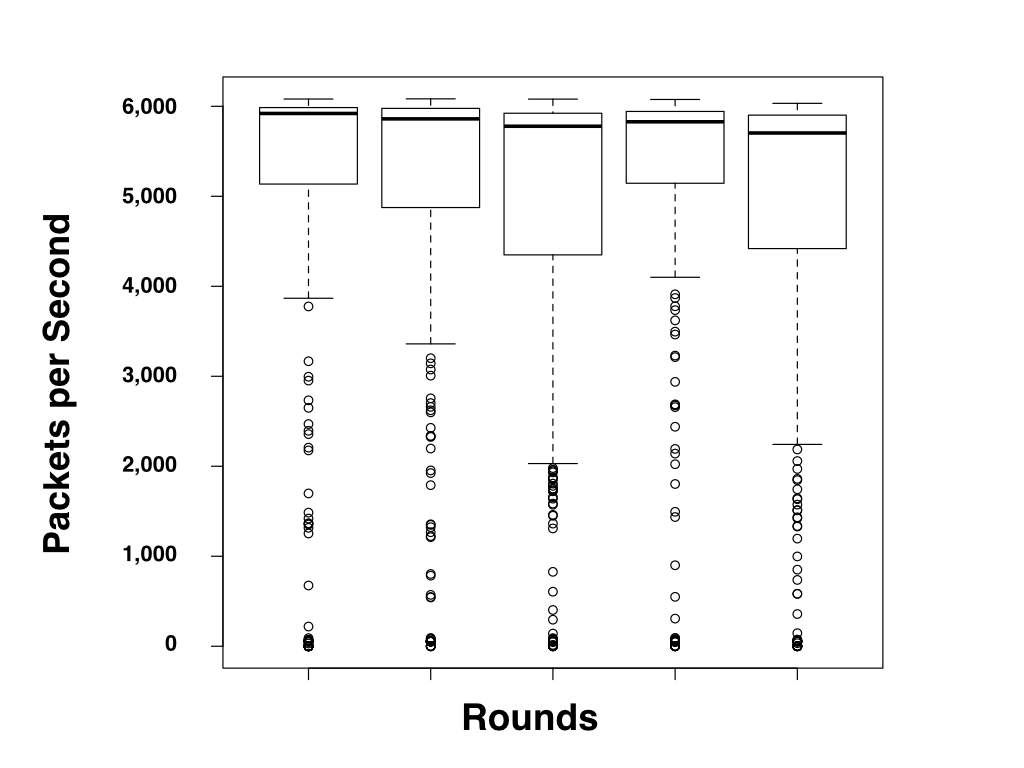
\includegraphics[width=2in]{authDCPPS}
    \label{fig:authDCPPS}
  \end{figure}
} 
\frame{
  \frametitle{Load on Domain Controller}
  \begin{figure}[H] \centering
    \caption[Test 1:  Domain Controller Metrics]{Domain controller CPU and
    memory utilization during the first test.}
    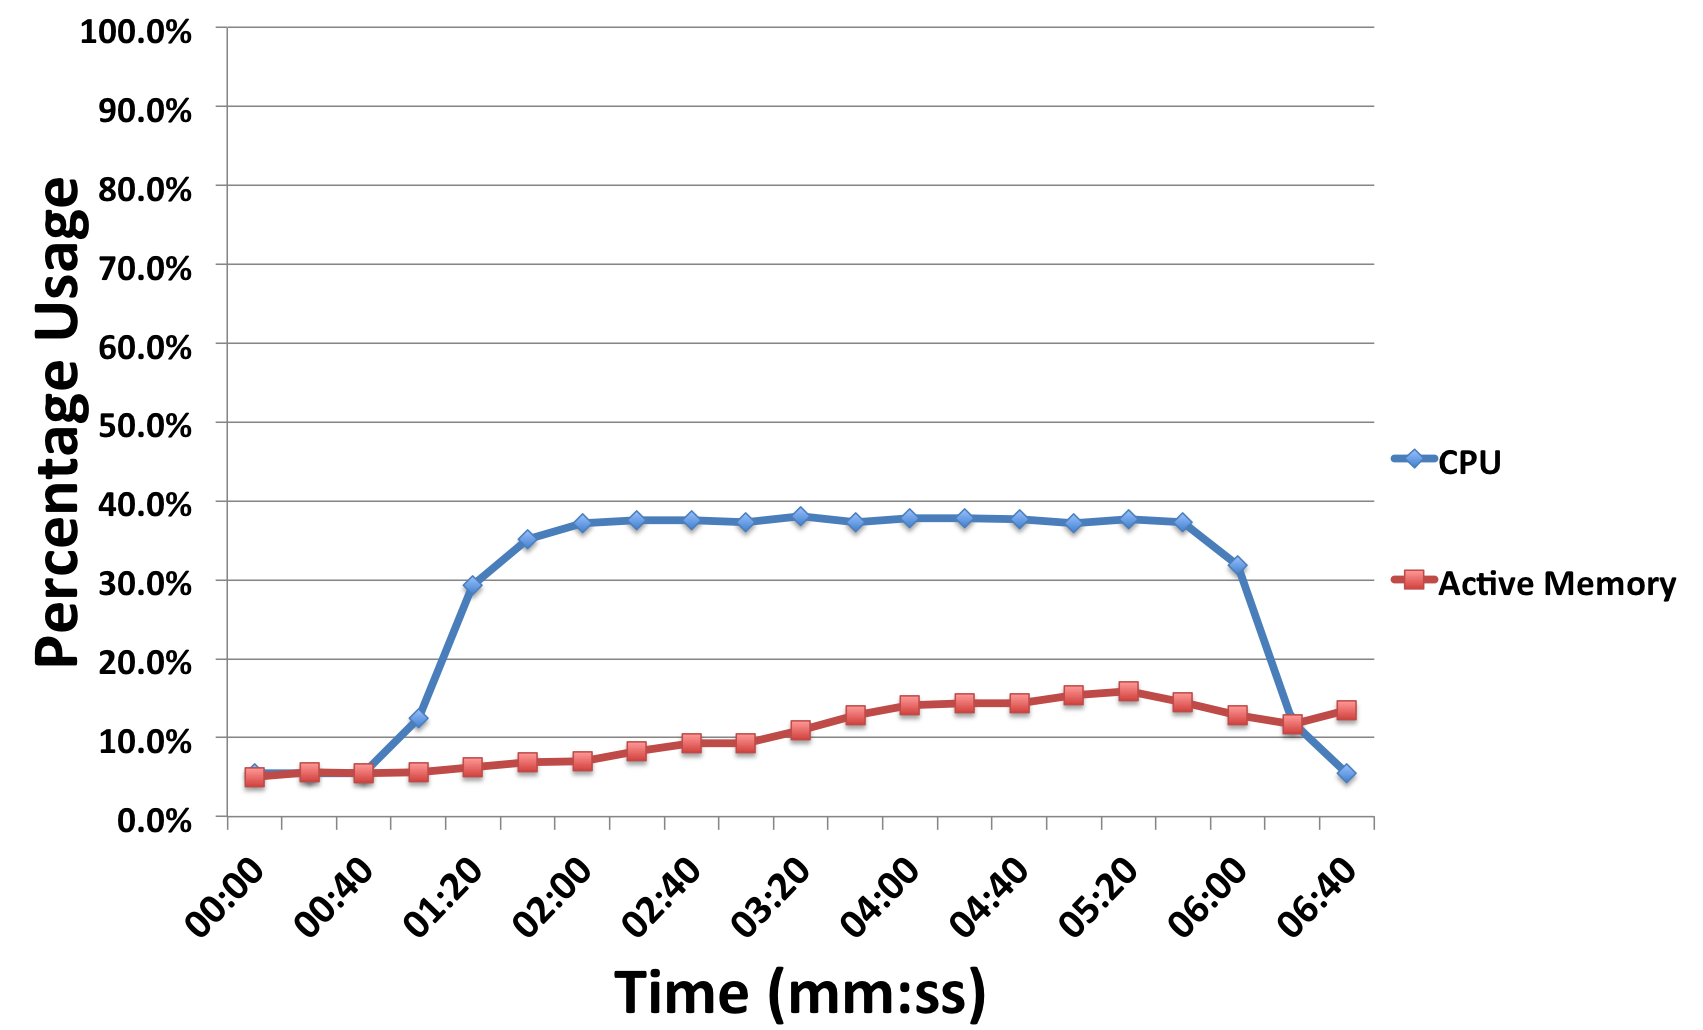
\includegraphics[width=2.8in]{authDCMetrics}
    \label{fig:authDCMetrics}
  \end{figure}
}

\subsection{Second Test}
\frame{
  \frametitle{Results}
  \begin{itemize}
  \item Not quite as successful as first
  \item Client machines were undersized compared to standard desktop computers
  in enterprise environment
  \item Result was that while they produced a sufficient amount of traffic,
  they would have been a little slow to use
  \item Solution:  Use more powerful client machines, or use during idle down
  times
  \end{itemize}
}
\frame{
  \frametitle{Results}
  \begin{figure}[H] \centering
    \caption[Test 2:  Client Metrics]{Client CPU and memory utilization during
    the second test.}
    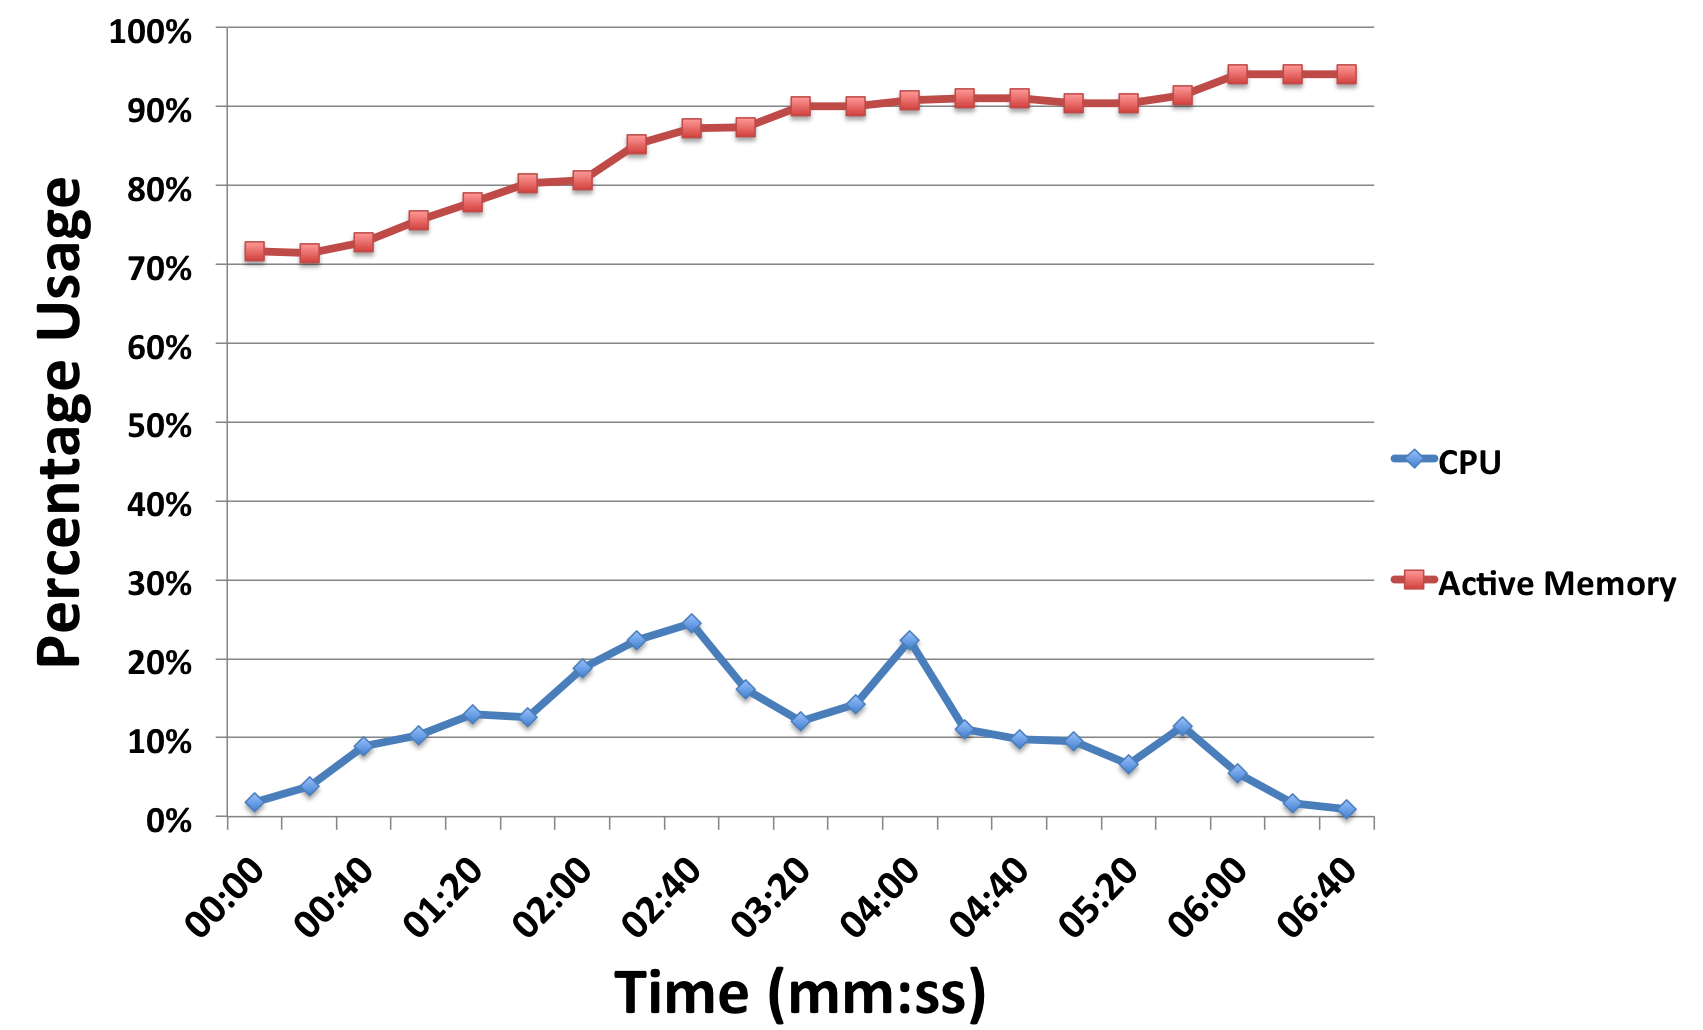
\includegraphics[width=2.8in]{allModsClientMetrics}
    \label{fig:allModsClientMetrics}
  \end{figure}
}

\section{Conclusion}
\frame{
  \frametitle{Future Work}
  \begin{itemize}
  \item Build-out tool
  \item Add new functionality like e-mail and printing support
  \item Give users more control over type of load generated
  \item Increase stochasticity to better simulate user behavior
  \end{itemize}
} 

\frame{
  \frametitle{Conclusion}
  \begin{itemize}
  \item Based on the results of our first test, D-PLG will meet our needs to
  implement AFP against a domain controller
  \item We believe our results demonstrate D-PLG's applicability to other
  problems that require dynamic traffic between unbounded network components
  \end{itemize}
} 

\frame{
  \frametitle{Summary}
  \tableofcontents
} 

\frame{
  \centering
  \Huge Questions?
} 

\frame[allowframebreaks]{
  \bibliography{../LoadGenerator}{}
  \bibliographystyle{plain}
} 

\end{document}
